\section{Methodology}

\label{sec:methodology}

We present MARAHS, a unified framework for safe autonomous drone operation in hurricane conditions. Figure~\ref{fig:architecture} shows the complete system architecture.

\begin{figure}[t]
\centering
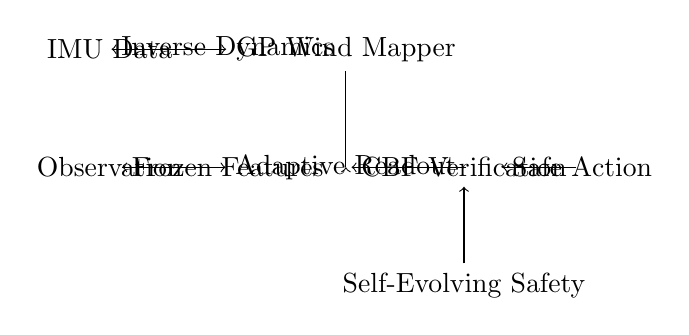
\begin{tikzpicture}[node distance=1.5cm]
    % Nodes
    \node (imu) {IMU Data};
    \node (wind) [right of=imu] {Inverse Dynamics};
    \node (gp) [right of=wind] {GP Wind Mapper};
    \node (obs) [below of=imu] {Observation};
    \node (feat) [right of=obs] {Frozen Features};
    \node (readout) [right of=feat] {Adaptive Readout};
    \node (cbf) [right of=readout] {CBF Verification};
    \node (action) [right of=cbf] {Safe Action};
    \node (ses) [below of=cbf] {Self-Evolving Safety};
    
    % Edges
    \draw[->] (imu) -- (wind);
    \draw[->] (wind) -- (gp);
    \draw[->] (obs) -- (feat);
    \draw[->] (feat) -- (readout);
    \draw[->] (readout) -- (cbf);
    \draw[->] (cbf) -- (action);
    \draw[->] (ses) -- (cbf);
    \draw[->] (gp) |- (readout);
\end{tikzpicture}
\caption{MARAHS Architecture. IMU data feeds wind estimation, which informs the GP wind mapper. Observations pass through frozen features to the adaptive readout, whose output is verified by the CBF before execution. The Self-Evolving Safety module discovers new constraints from near-miss experiences.}
\label{fig:architecture}
\end{figure}

\subsection{System Dynamics}

Consider a quadrotor UAV with state $x = [p^\top, v^\top]^\top \in \mathbb{R}^6$ where $p \in \mathbb{R}^3$ is position and $v \in \mathbb{R}^3$ is velocity. The dynamics are control-affine:
\begin{equation}
    \dot{x} = f(x) + g(x)u + w(x,t)
\end{equation}
where $f(x) = [v^\top, (F_{\text{grav}} + F_{\text{drag}})^\top/m]^\top$ represents drift dynamics, $g(x) \in \mathbb{R}^{6 \times 4}$ is the control input matrix, $u \in [-1,1]^4$ is the control action, and $w(x,t) \in \mathbb{R}^6$ is the wind disturbance.

\subsection{Safety Constraints}

We define the safe set $\mathcal{S}$ via barrier functions $h_i(x) \geq 0$:
\begin{equation}
    \mathcal{S} = \{x \in \mathbb{R}^6 : h_i(x) \geq 0, \forall i \in \{1, \ldots, m\}\}
\end{equation}
where the constraints include altitude ($h_{\text{alt}}$), velocity ($h_{\text{vel}}$), attitude ($h_{\text{tilt}}$), and inter-agent separation ($h_{\text{sep}}$).

\subsection{Control Barrier Functions}

A Control Barrier Function (CBF) $h: \mathbb{R}^6 \to \mathbb{R}$ provides safety guarantees if:
\begin{equation}
    \dot{h}(x) \geq -\alpha(h(x))
\end{equation}
for all $x \in \mathcal{S}$, where $\alpha$ is a class-$\mathcal{K}$ function. This ensures forward invariance of the safe set~\cite{ames2014control}.

\subsection{Online Gaussian Process Wind Mapping}

\label{sec:gp_wind}

We model the wind field as a Gaussian Process:
\begin{equation}
    w(x) \sim \mathcal{GP}(m(x), k(x, x'))
\end{equation}
where $m(x)$ is a Rankine vortex prior and $k(x, x')$ is a Matérn 5/2 kernel with Automatic Relevance Determination:
\begin{equation}
    k(x, x') = \sigma_f^2 \left(1 + \frac{\sqrt{5}r}{l} + \frac{5r^2}{3l^2}\right) \exp\left(-\frac{\sqrt{5}r}{l}\right)
\end{equation}
where $r = \|x - x'\|$ and $l$ is the length scale.

The online update uses the Woodbury identity to maintain $O(n^2)$ complexity per observation.

\subsection{Safety-Verified Meta-Adaptation}

\label{sec:adaptation}

The Neural Fly architecture~\cite{dean2022neural} adapts a linear readout layer online via Recursive Least Squares (RLS):
\begin{align}
    z_t &= \phi(x_t) \quad \text{(frozen features)} \\
    y_t &= W_t z_t + b_t \quad \text{(adaptive readout)} \\
    W_{t+1} &= W_t + K_t(a_t - y_t)z_t^\top \quad \text{(RLS update)}
\end{align}

\textbf{Novel contribution:} We verify that the adapted controller satisfies CBF constraints before execution. Define the \emph{safe adaptation cone}:
\begin{equation}
    \mathcal{C}_{\text{safe}} = \{\Delta u : \nabla h_i \cdot g(x) \cdot \Delta u \geq -h_i(x) - \alpha(h_i(x)) + \nabla h_i \cdot g(x) \cdot u_{\text{orig}}, \forall i\}
\end{equation}

If $\Delta u \in \mathcal{C}_{\text{safe}}$, then $u_{\text{adapted}} = u_{\text{orig}} + \Delta u$ satisfies all CBF conditions (Theorem~\ref{thm:adaptation_safety}).

\subsection{IMU-to-Wind Inverse Dynamics}

\label{sec:wind}

We estimate wind forces from IMU measurements by solving the inverse dynamics problem:
\begin{equation}
    a_{\text{wind}} = a_{\text{measured}} - a_{\text{gravity}} - a_{\text{thrust}} - a_{\text{drag}}
\end{equation}
where each component is estimated from motor commands and the aerodynamic model.

\subsection{Adversarial Safety Verification}

\label{sec:adversarial}

We find the worst-case perturbation $\delta^*$ that maximizes safety violation:
\begin{equation}
    \delta^* = \arg\max_{\|\delta\| \leq \epsilon} \left[-\min_i h_i(x, u + \delta)\right]
\end{equation}

This is solved via projected gradient ascent with multiple random restarts.

\subsection{Information-Theoretic Coverage}

\label{sec:information}

We maximize mutual information about the wind field:
\begin{equation}
    \pi^* = \arg\max_{\pi \in \mathcal{P}} \sum_{t=1}^T \gamma^t I(w; z_t | z_{1:t-1})
\end{equation}
where $I(w; z_t | z_{1:t-1})$ is the conditional mutual information and $\gamma$ is the discount factor.

\subsection{Multi-Scale Adaptation}

\label{sec:multiscale}

We formalize adaptation at four timescales with a Lyapunov composition:
\begin{equation}
    V_{\text{total}} = \sum_{i=1}^4 \alpha_i V_i(\theta_i)
\end{equation}
where $\theta_i$ are parameters at timescale $i$ and $V_i$ are individual Lyapunov functions.

\subsection{Self-Evolving Safety}

\label{sec:ses}

The Self-Evolving Safety (SES) system discovers new constraints from experience:
\begin{enumerate}
    \item \textbf{Detect} near-miss events where $\min_i h_i(x) < \delta$
    \item \textbf{Cluster} near-misses by root cause using distance-based clustering
    \item \textbf{Propose} new exclusion-zone constraints for each cluster
    \item \textbf{Verify} necessity (catches real failures) and sufficiency (prevents future failures)
    \item \textbf{Add} verified constraints to the CBF
\end{enumerate}

This is the first system that learns \emph{what} to be safe about, not just \emph{how} to be safe.
